\chapter{System Implementation, Testing and Validation}

\section{Introduction}
This chapter describes how Traxis was realized. Traxis's implementation, testing and validation was to make sure that it meets its set
objectives and the requirement specifications that were identified.

\section{System Implementation}
This section gives an overview of the project implementation. It highlights
the major components and the operation of the system as well as the different
user interfaces and activities that allow users to interact with the system.

\subsection{Implementation tools}
The Traxis system was implemented using a modern, scalable technology stack selected to ensure performance, reliability, and adaptability within the Ugandan transport context.

\textbf{Flutter (Dart)}
The mobile application was developed using Flutter, a cross-platform UI framework by Google, alongside the Dart programming language. Flutter enabled the development of a single codebase that runs on both Android and iOS devices, reducing development time and maintenance effort. Its widget-based architecture supported the creation of responsive and user-friendly interfaces suitable for a wide range of devices, including low and mid-range smartphones commonly used in Uganda.

\textbf{Django and Django REST Framework (DRF)}
The backend system was implemented using Django, a high-level Python web framework, together with the Django REST Framework for API development. Django handled business logic, request processing, and system coordination, while DRF exposed RESTful APIs that facilitated secure communication between the mobile applications, admin portal, and external services.

\textbf{PostgreSQL (with PostGIS)}
PostgreSQL was used as the primary relational database for persistent data storage. It provided strong data integrity, reliability, and support for complex queries. The PostGIS extension enabled geospatial data processing, which was essential for location-based features such as route mapping, nearest-vehicle identification, and geographic queries.

\textbf{Firebase Services}
Firebase was integrated to support real-time features and user management:

Firebase Authentication was used for secure user registration and login, particularly through phone-number-based authentication, which aligns with local user accessibility.
Firebase Cloud Messaging (FCM) enabled real-time push notifications, such as booking confirmations, trip updates, and alerts for both passengers and drivers.

\textbf{Google Maps API}
The Google Maps Platform was used to provide mapping, navigation, and geolocation services. It enabled real-time vehicle tracking, route visualization, and distance calculations, improving user interaction and operational coordination within the system.

\textbf{AWS (Amazon Web Services)}
AWS was utilized for compute-intensive operations such as transcription and other backend processing tasks. Its scalable cloud infrastructure ensured efficient handling of resource-demanding processes without affecting overall system performance.

\textbf{MCP (Model Control Protocol)}
MCP was integrated to support AI-driven functionalities, including predictive analytics and intelligent system behavior. Implemented using Python, it enabled advanced features such as demand forecasting and improved coordination between passengers and shuttle operators.

\textbf{Hive and Background Sync Mechanisms}
Hive, a lightweight local database for Flutter, was used to support offline functionality. Combined with background synchronization tools, it allowed the system to queue actions performed offline and automatically sync them once network connectivity was restored—an essential feature for areas with unstable internet access.

\textbf{Vue.js (Admin Portal)}
The Admin Portal was developed using Vue.js, a progressive JavaScript framework. It provided administrators with a responsive interface for managing users, monitoring trips, viewing analytics, and configuring system settings. Its reactive architecture enabled real-time updates and efficient interaction with backend APIs.

\subsection{User interface design}
The system can be launched from the phone just like any other Android or IOS
applications and after it has been launched, a login interface appears. This
is helpful in authenticating users
\subsubsection{Account Creation}
Passengers can create an account by providing their phone number and a next of kin's phone number, which is verified through a one-time password (OTP) sent via SMS. Operators are asked to provide an E-mail address in addition to their phone number. This method ensures a secure and straightforward registration process, particularly suited for users in Uganda who may not have access to email-based authentication.

\subsubsection{Operator Actions}
Once logged in, operators can access the main dashboard, which provides options for booking rides, viewing trip history, and managing their profiles. The interface is designed to be intuitive and user-friendly, with clear navigation and accessible features. Operators can register a company, the number of vehicles they have,the routes they operate on, and how much they charge for specific routes. They can also view and manage their bookings and indicate whether or not they support parcel delivery. On the dashboard, they can also view the number of passengers that have booked rides with them and the total revenue earned. They can add new vehicles to their fleet and view the details of their vehicles such as their location during trips and the number of trips they have made. Operators can also view the details of their passengers such as their name, phone number, and next of kin's phone number. They can also view the details of their trips such as the route taken, the distance covered, and the fare charged. 

\begin{figure}[htbp]
\centering

\begin{subfigure}{0.32\textwidth}
    \centering
    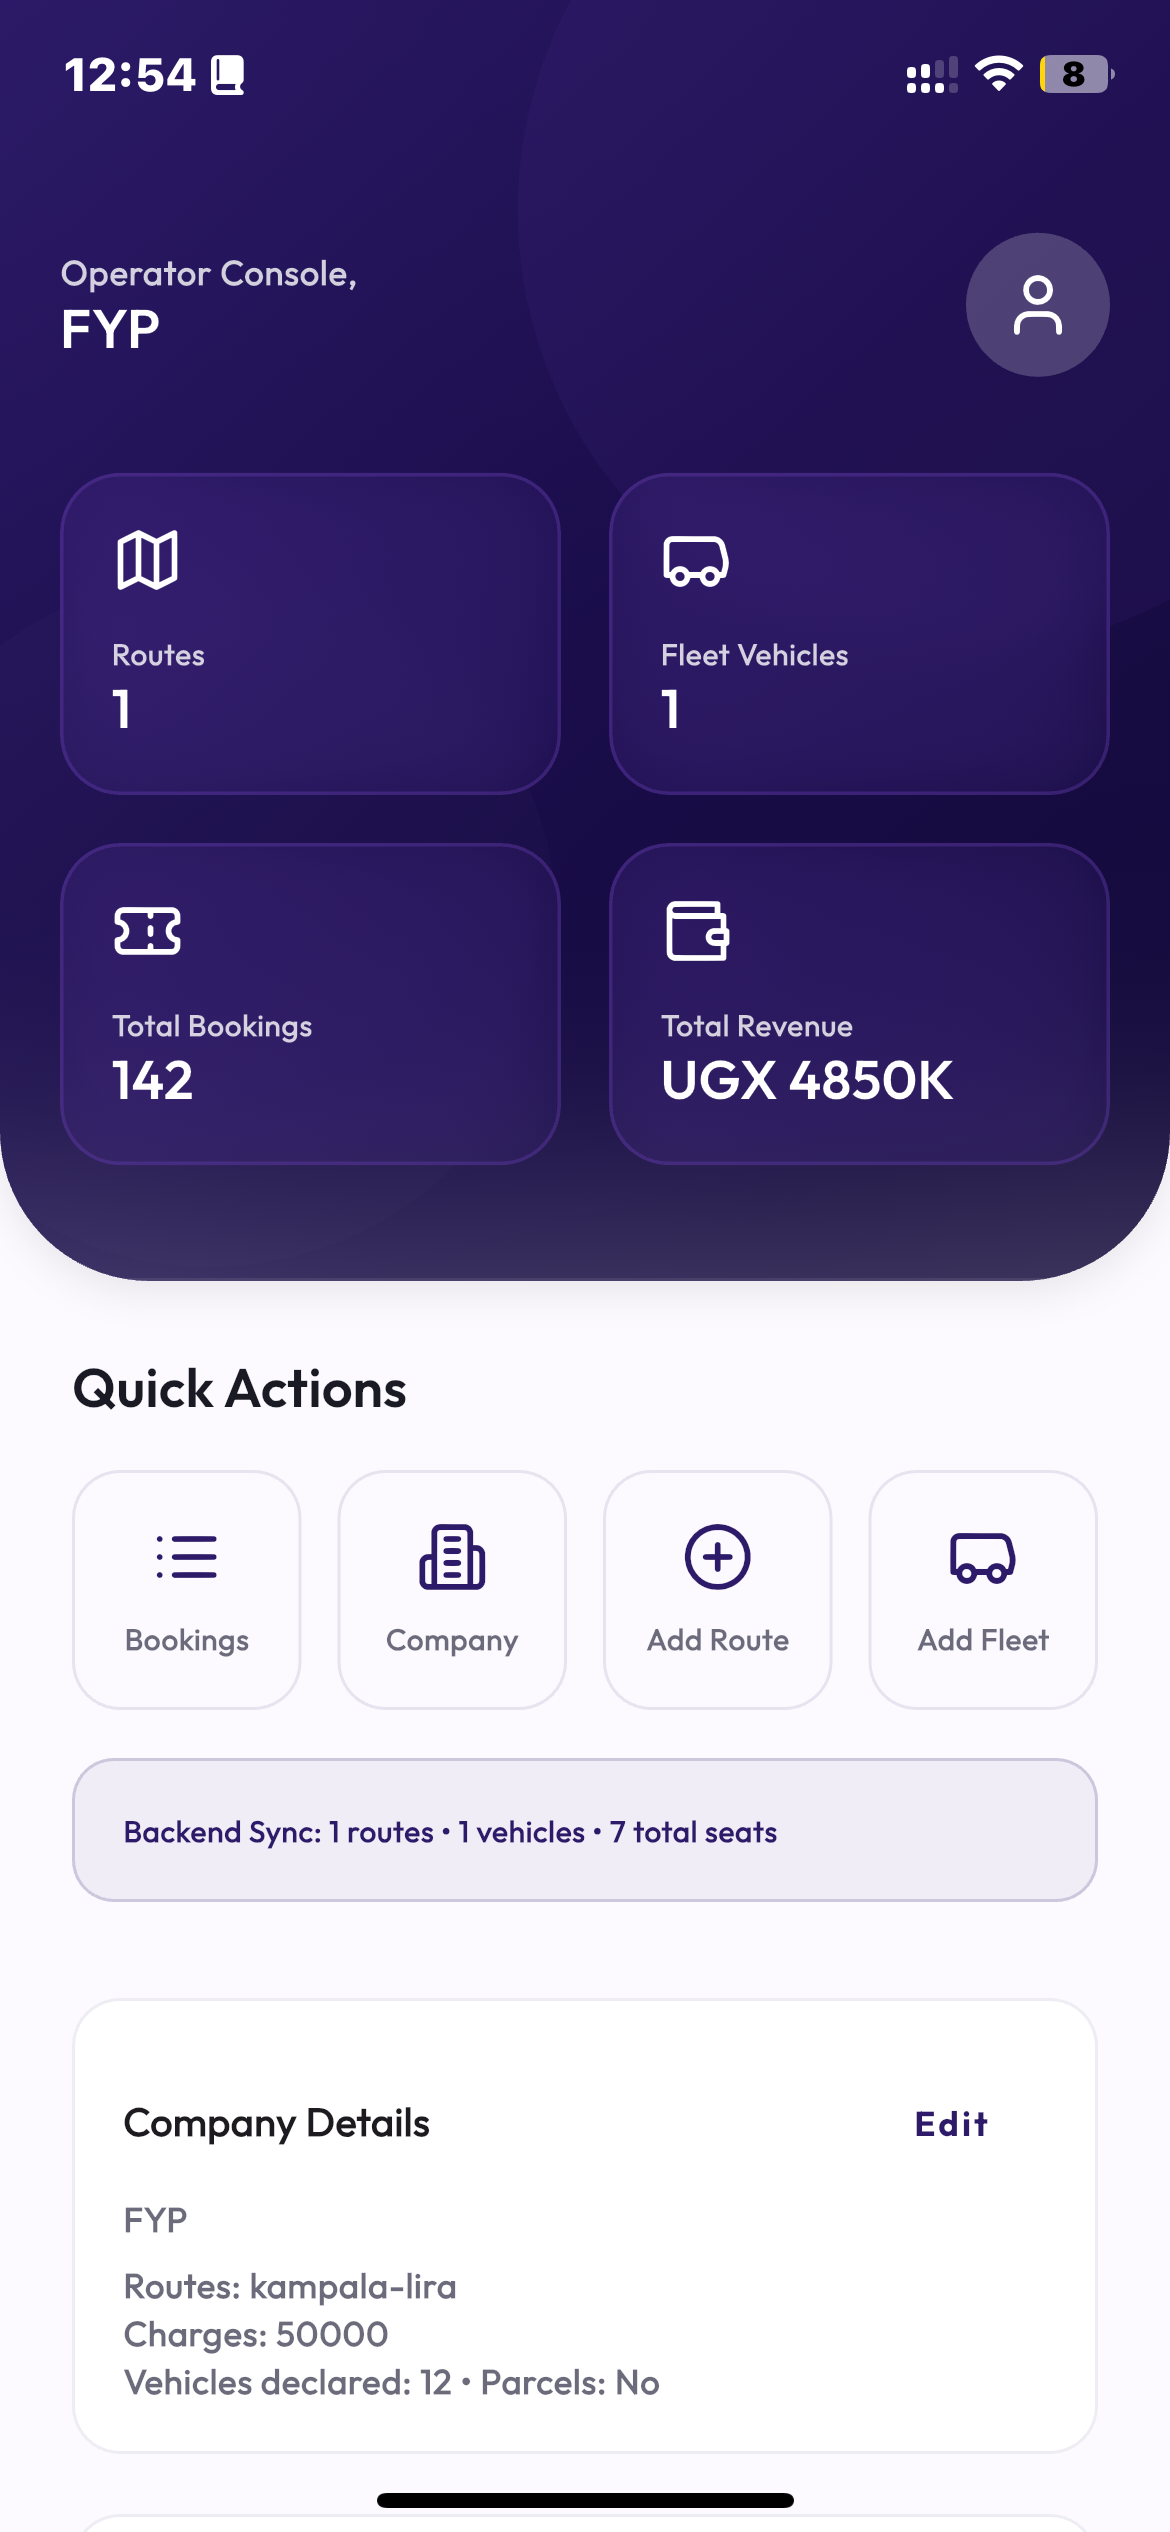
\includegraphics[width=\linewidth]{images/FYP/Operator dashboard.PNG}
    \caption{Operator dashboard}
\end{subfigure}
\hfill
\begin{subfigure}{0.32\textwidth}
    \centering
    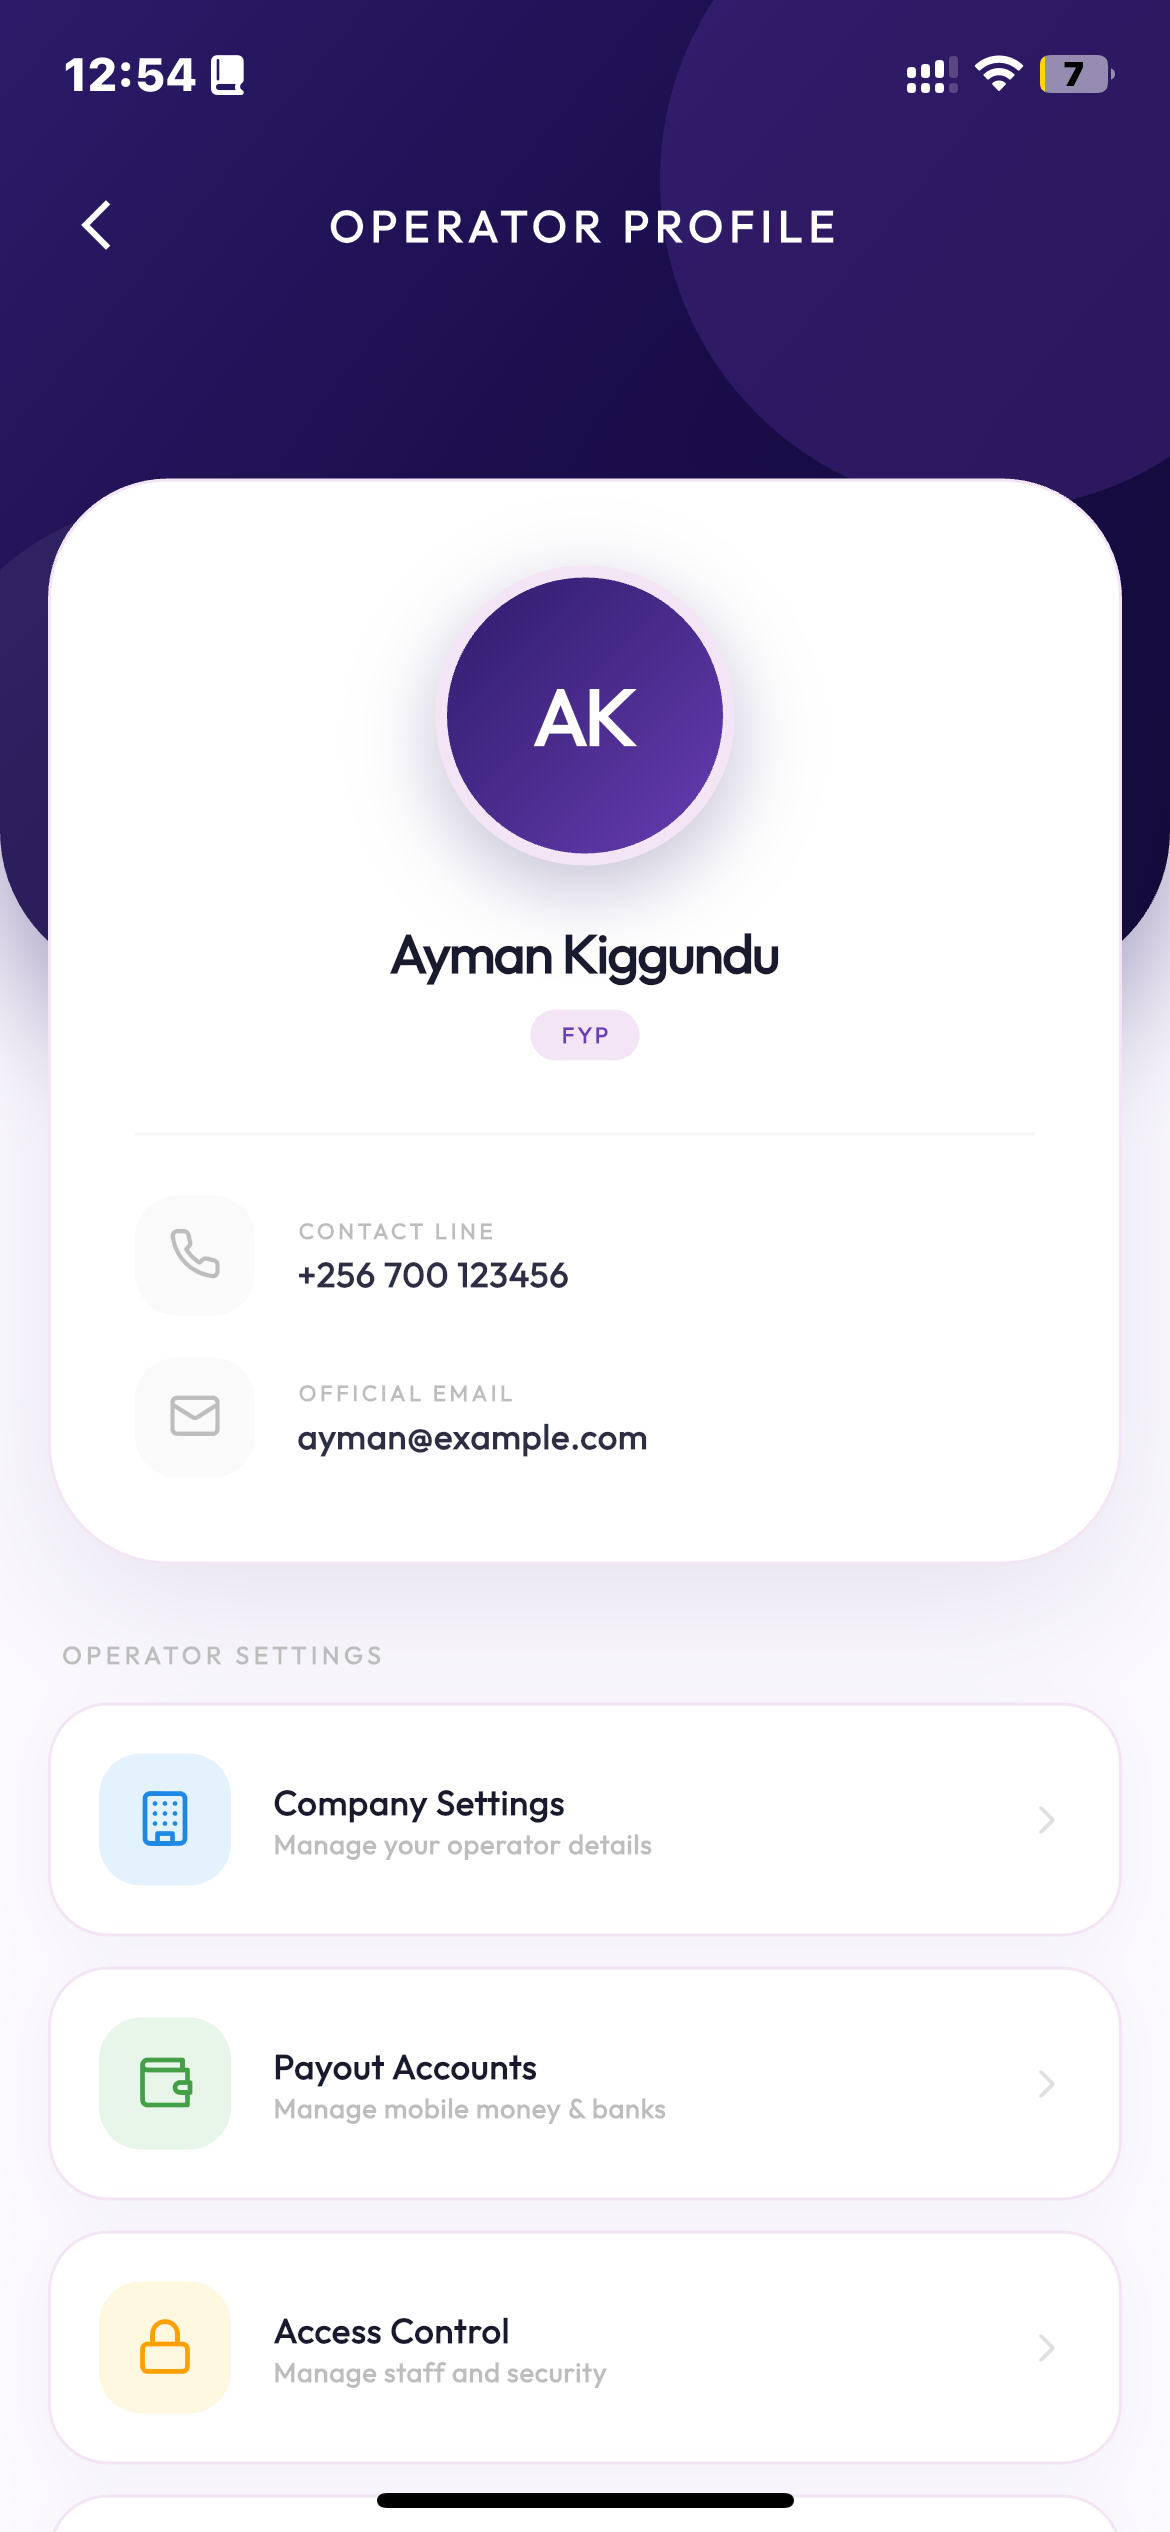
\includegraphics[width=\linewidth]{images/FYP/Operator profile.PNG}
    \caption{Operator profile}
\end{subfigure}
\hfill
\begin{subfigure}{0.32\textwidth}
    \centering
    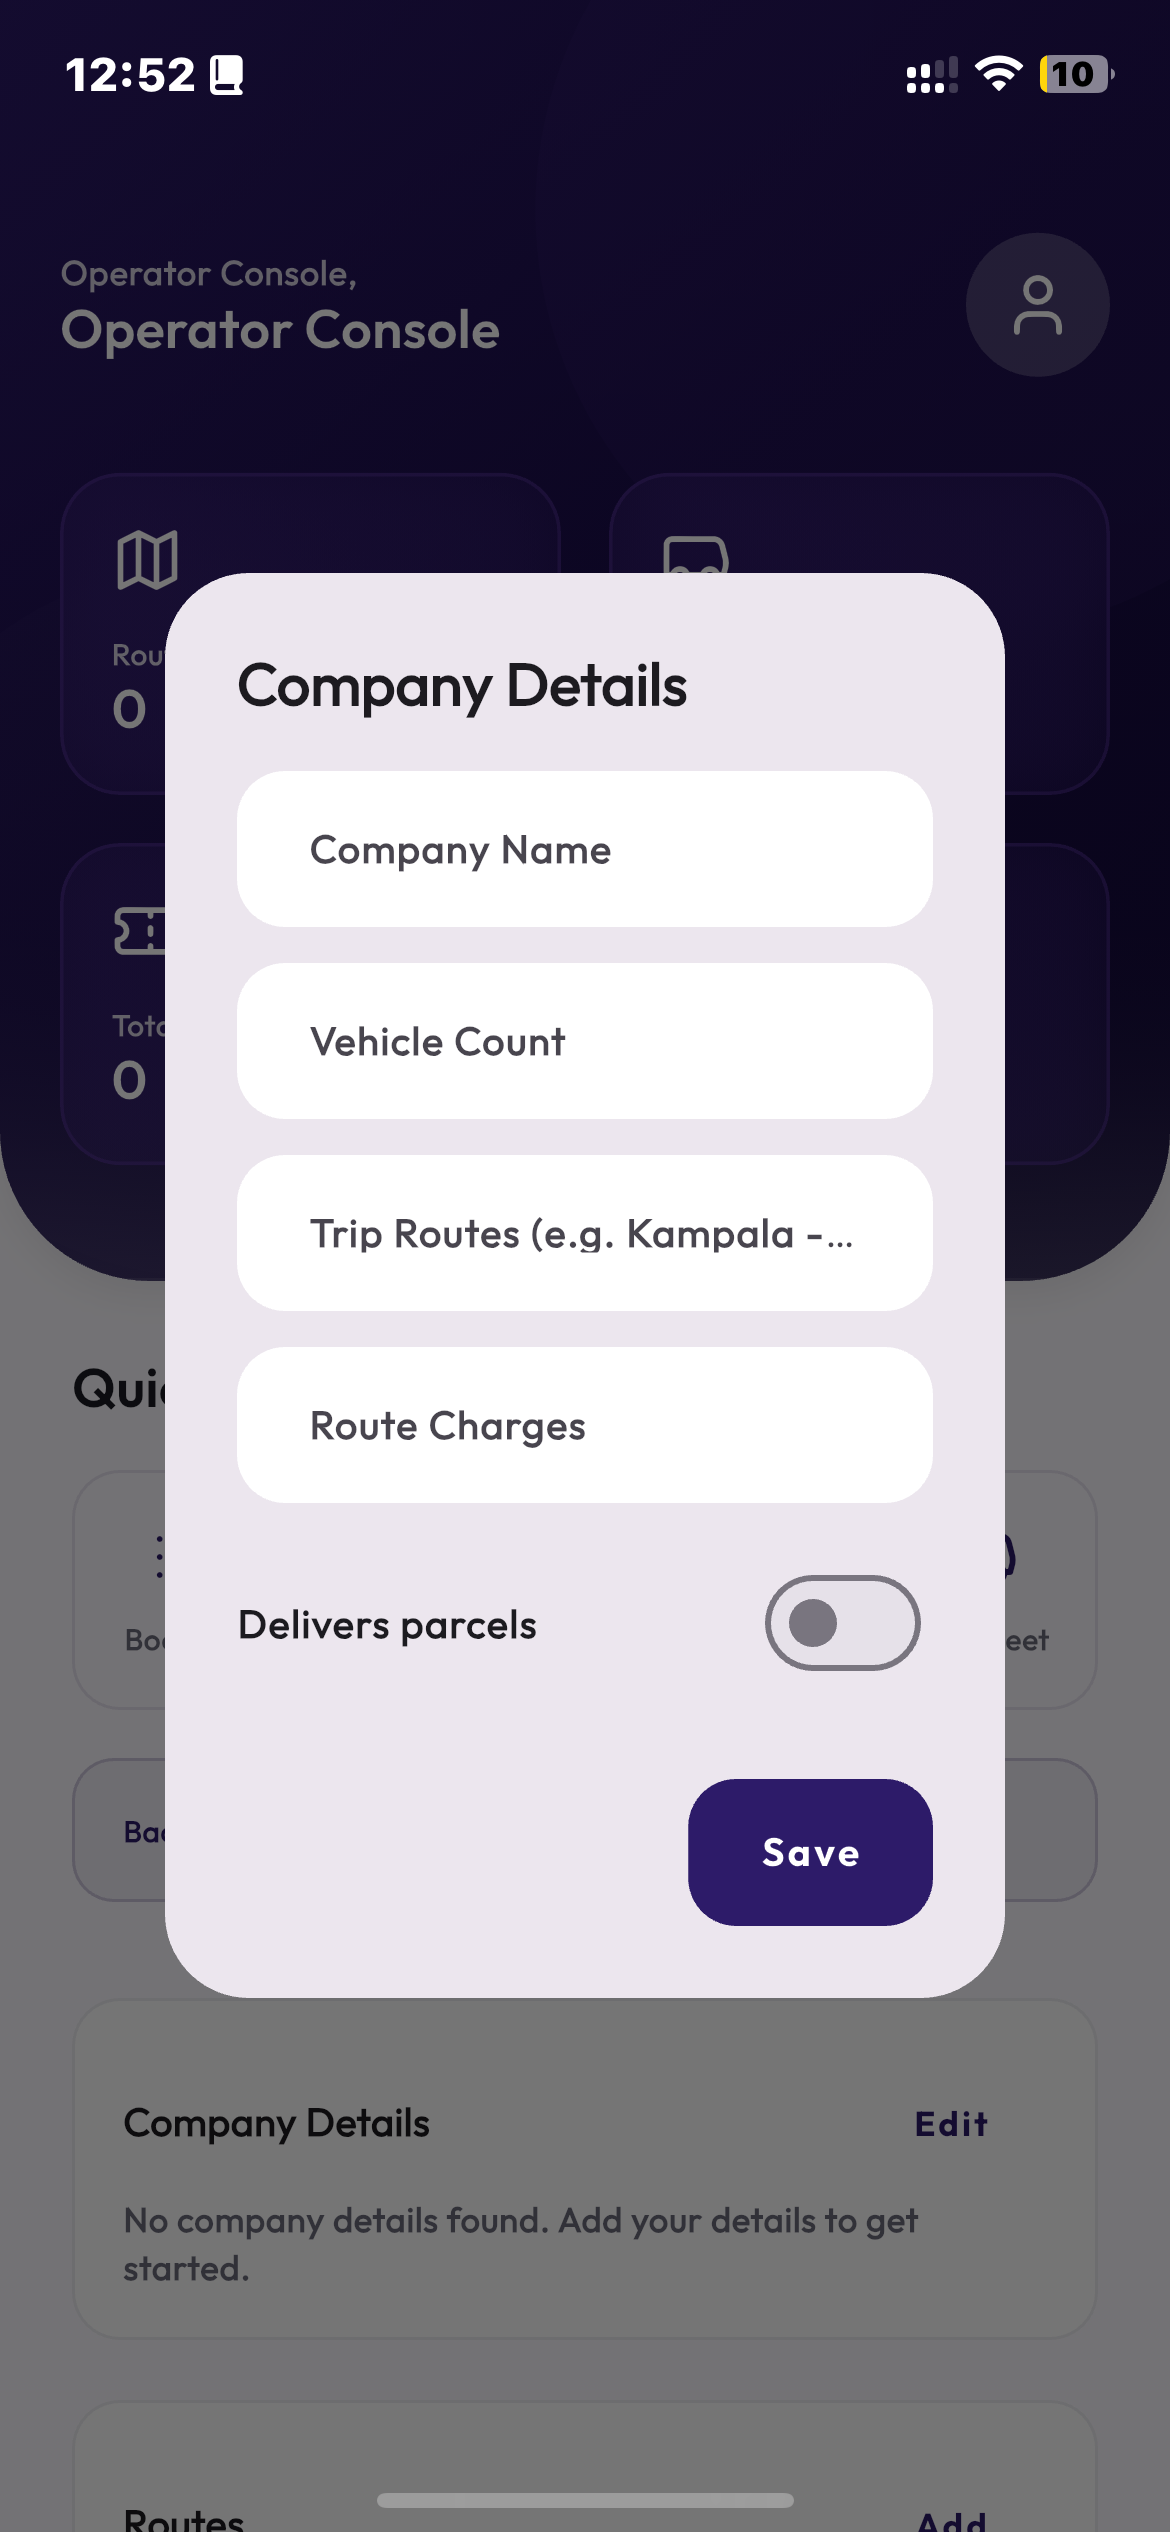
\includegraphics[width=\linewidth]{images/FYP/Company registration.PNG}
    \caption{Company registration}
\end{subfigure}

\caption{Operator interfaces}
\label{fig:operator-interfaces}

\end{figure}

\subsubsection{Passenger Actions}
Passengers can book rides by their pickup and drop-off locations, choosing a route, choose a dispatcher and confirming their booking. Passengers can also choose to book a ride for a future date and time.The app allows them to choose a seat in the taxi. The app provides a ticketing system that generates a unique ticket for each booking, which passengers can use to verify their ride and access the shuttle.During the trip, they can track the location of their shuttle in real-time and view the estimated time of arrival. They can also view their trip history, upcoming trips, and manage their profiles. The interface is designed to be simple and accessible, ensuring that users of varying technological proficiency can easily navigate and utilize the app's features. 
For parcel delivery, passengers can specify the pickup and drop-off locations, the type of parcel, the item's weight and even call for clarity on the fare to be charged. They can also track the status of their parcel in real-time and receive notifications about the delivery progress.


\begin{figure}[htbp]
\centering

\begin{subfigure}{0.32\textwidth}
    \centering
    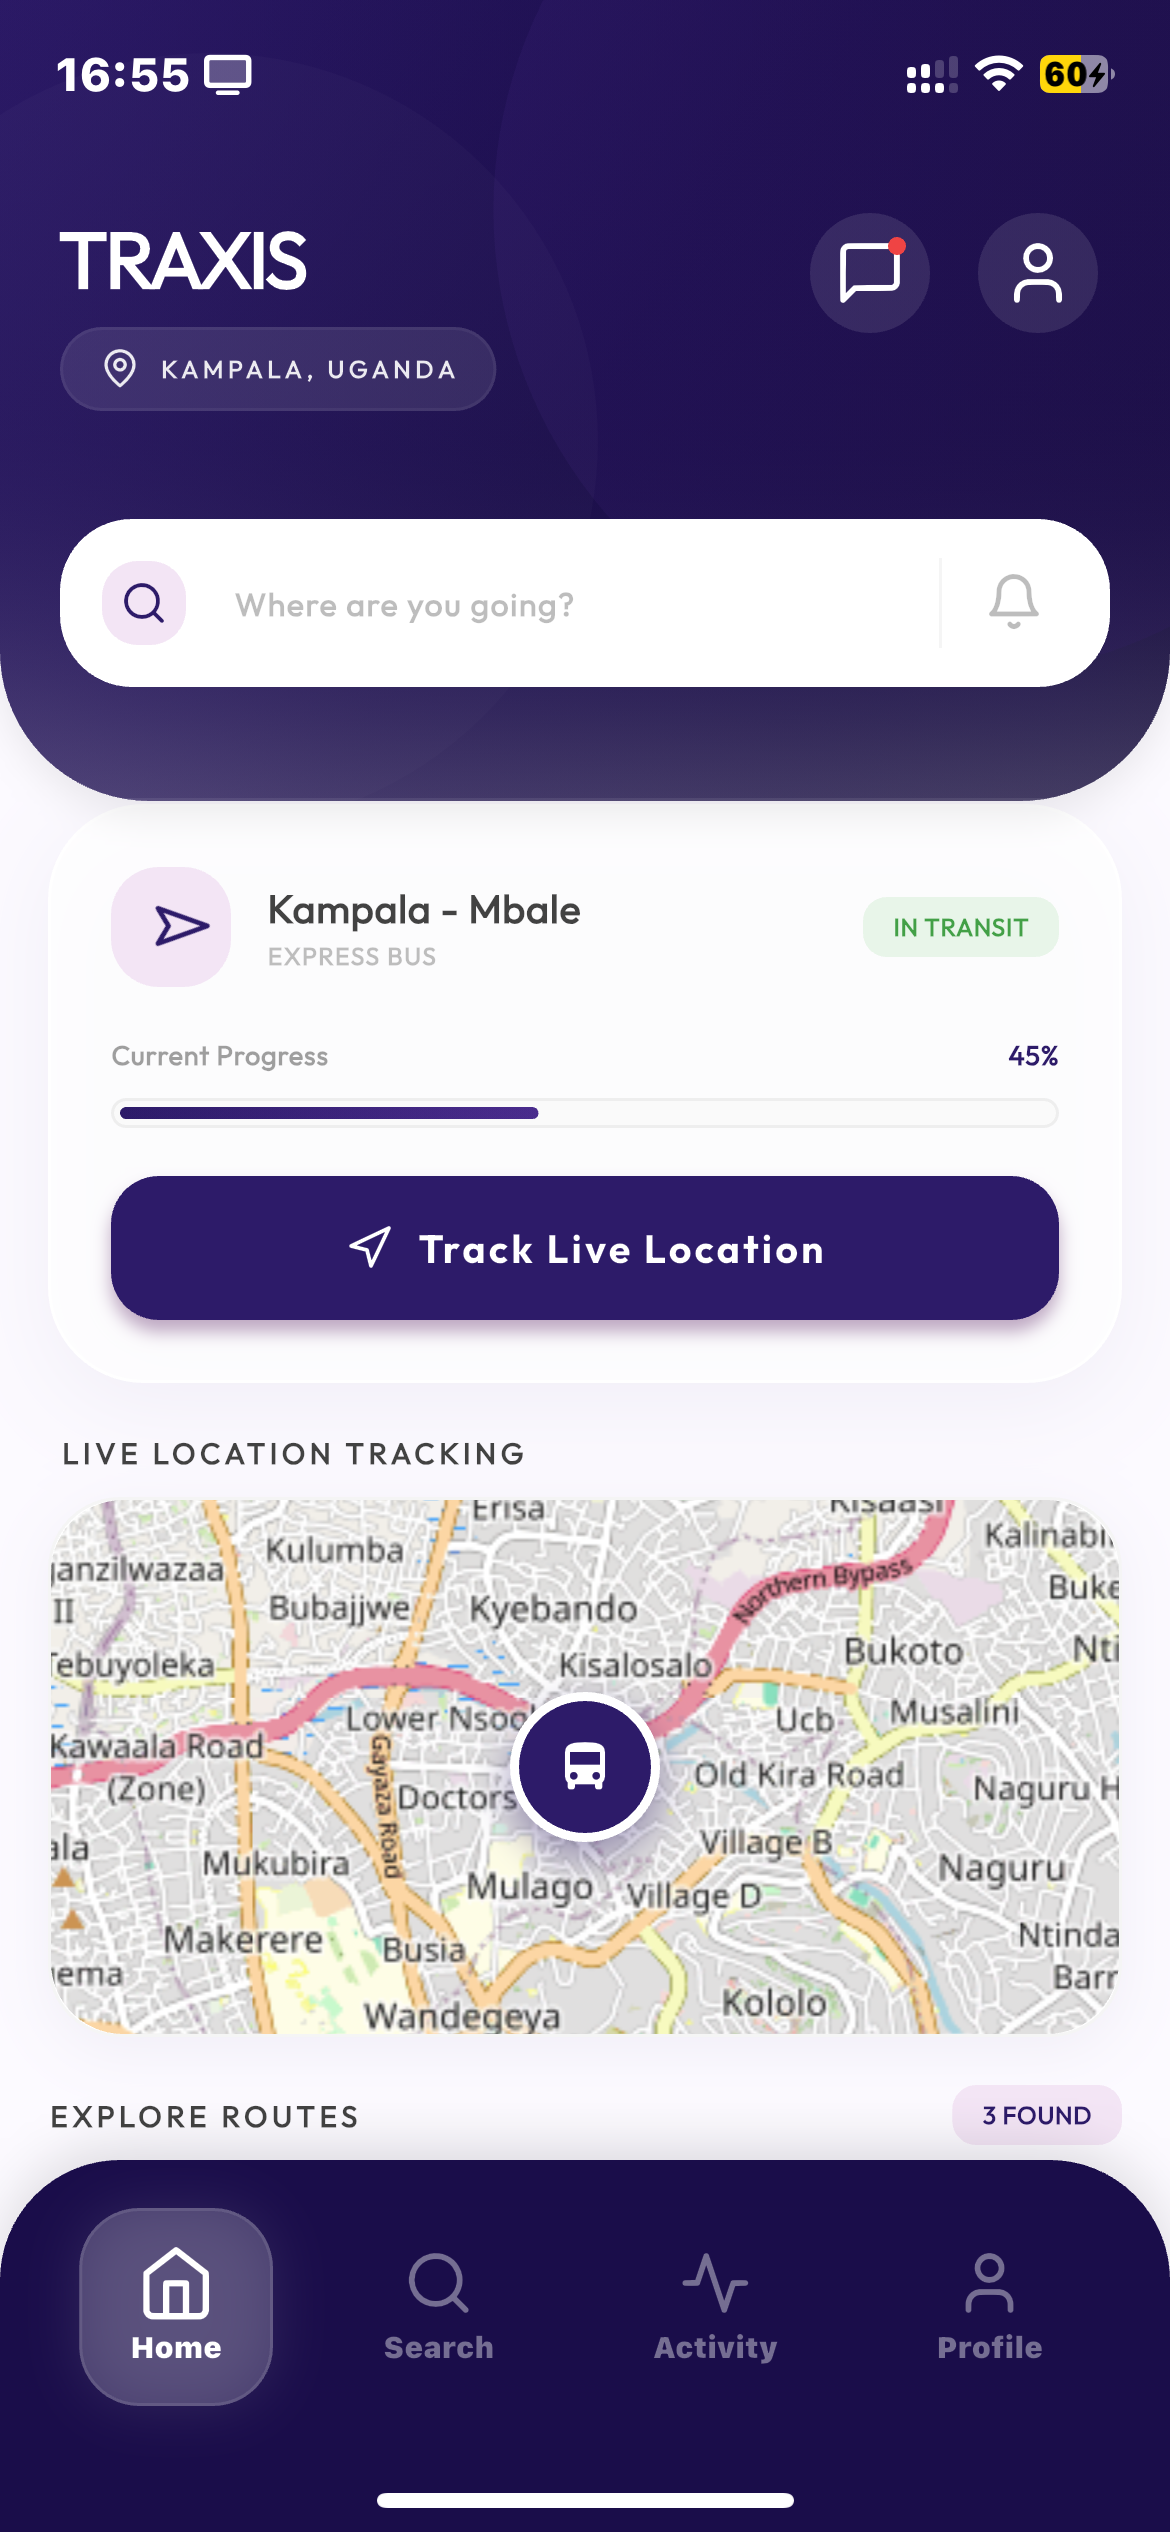
\includegraphics[width=\linewidth]{images/FYP/Passenger dashboard.PNG}
    \caption{Passenger dashboard}
\end{subfigure}
\hfill
\begin{subfigure}{0.32\textwidth}
    \centering
    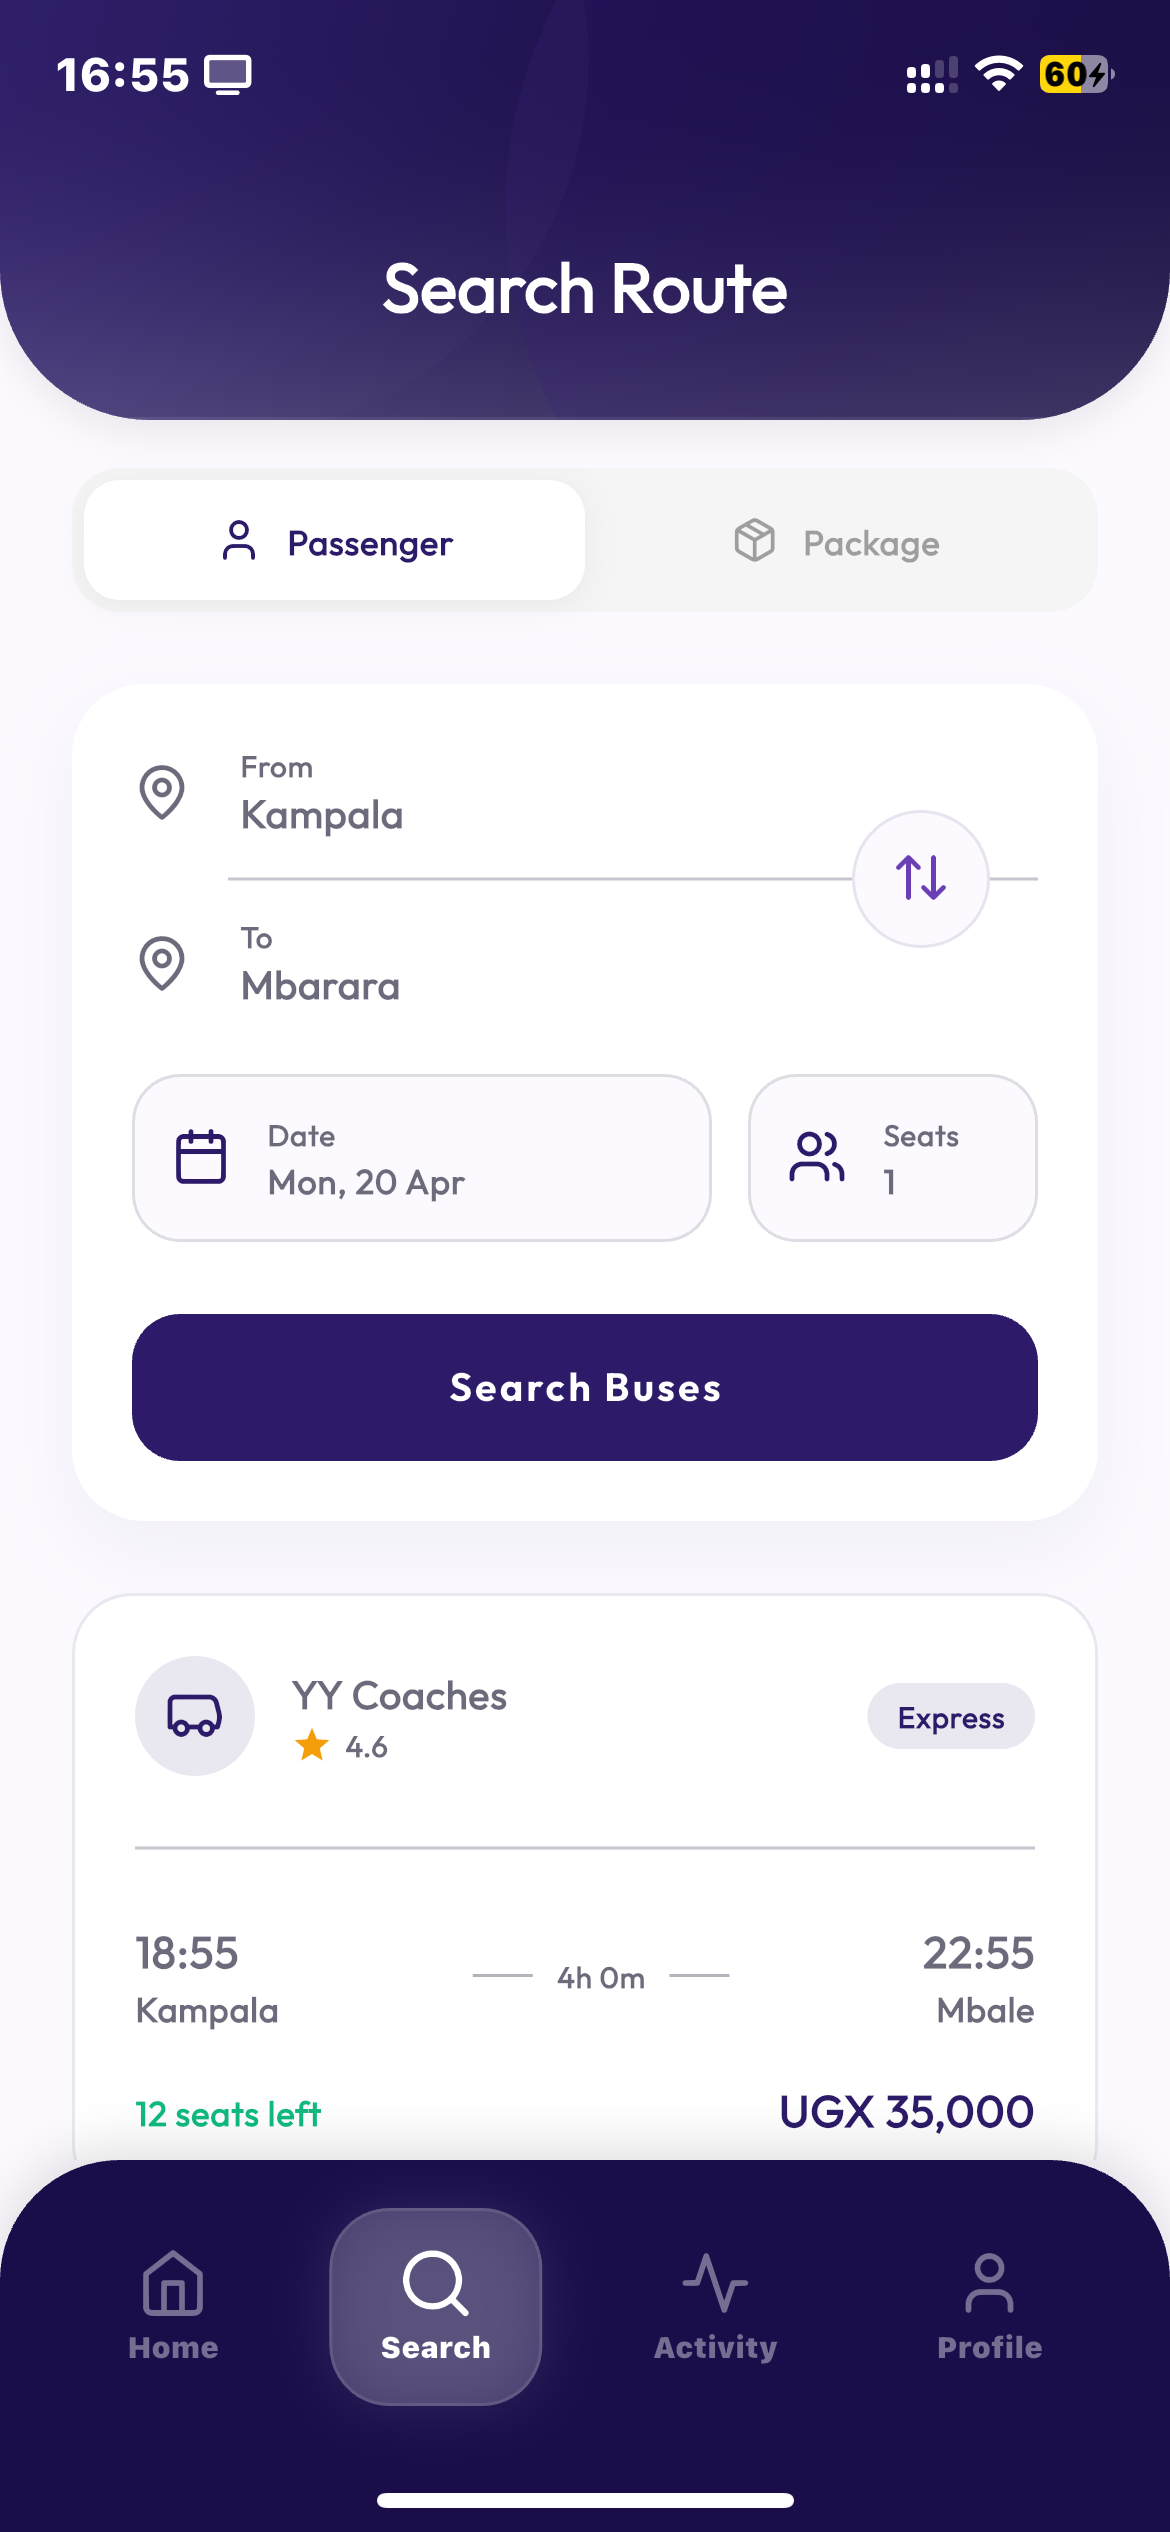
\includegraphics[width=\linewidth]{images/FYP/Route details.PNG}
    \caption{Imputting route details}
\end{subfigure}
\hfill
\begin{subfigure}{0.32\textwidth}
    \centering
    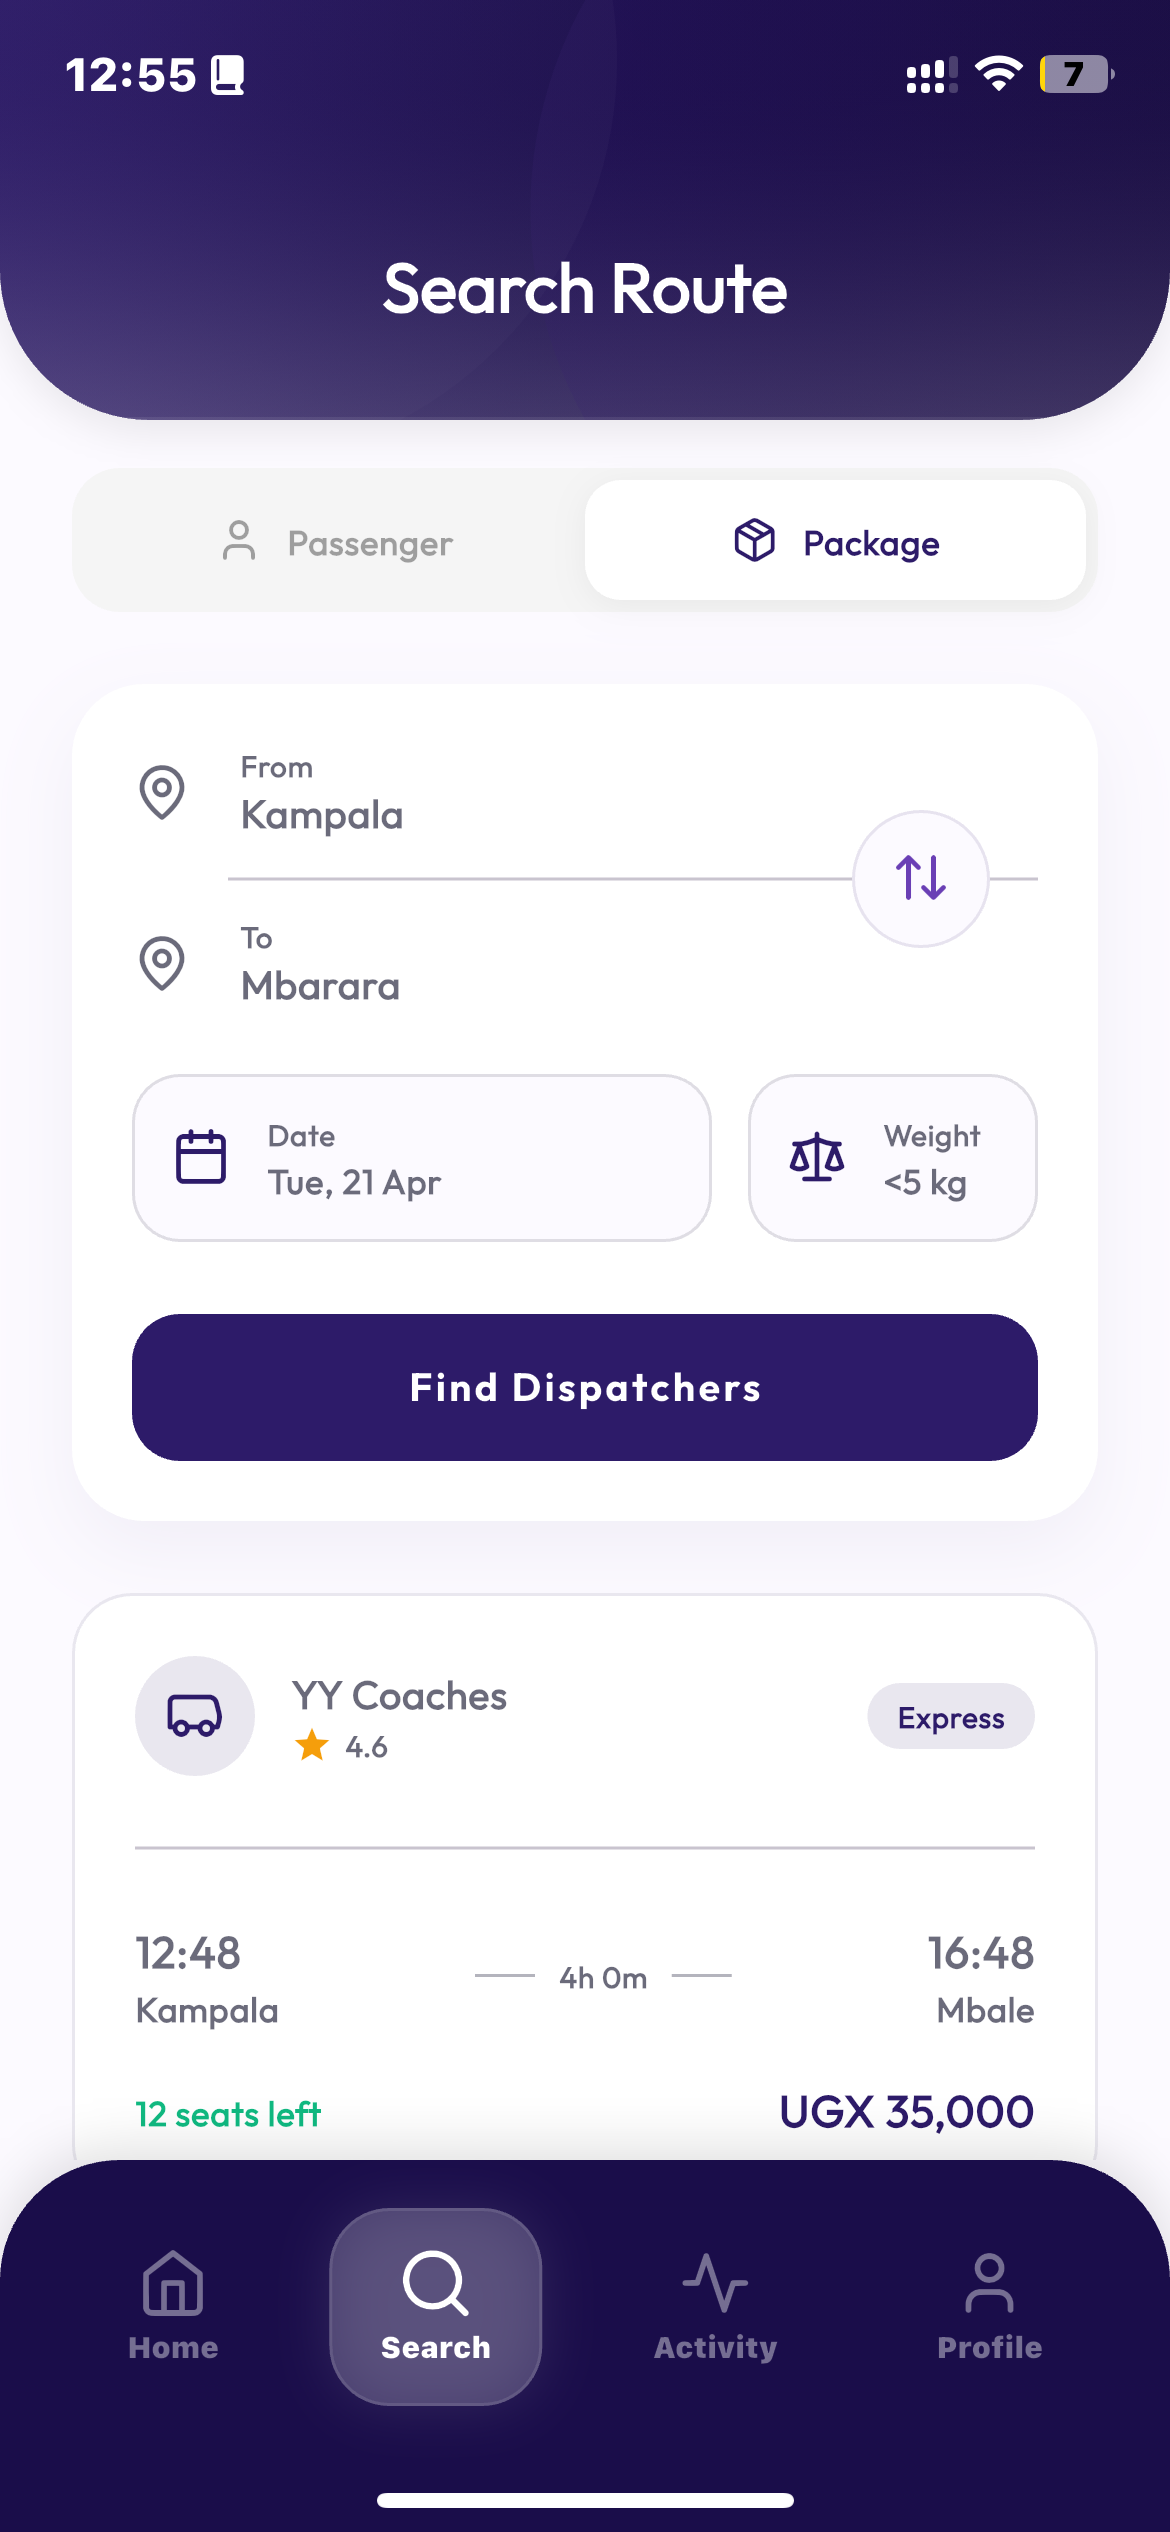
\includegraphics[width=\linewidth]{images/FYP/Parcel delivery details.PNG}
    \caption{Imputting parcel delivery details}
\end{subfigure}

\caption{Operator interfaces}
\label{fig:passenger-interfaces}

\end{figure}

\begin{figure}[htbp]
\centering

\begin{subfigure}{0.32\textwidth}
    \centering
    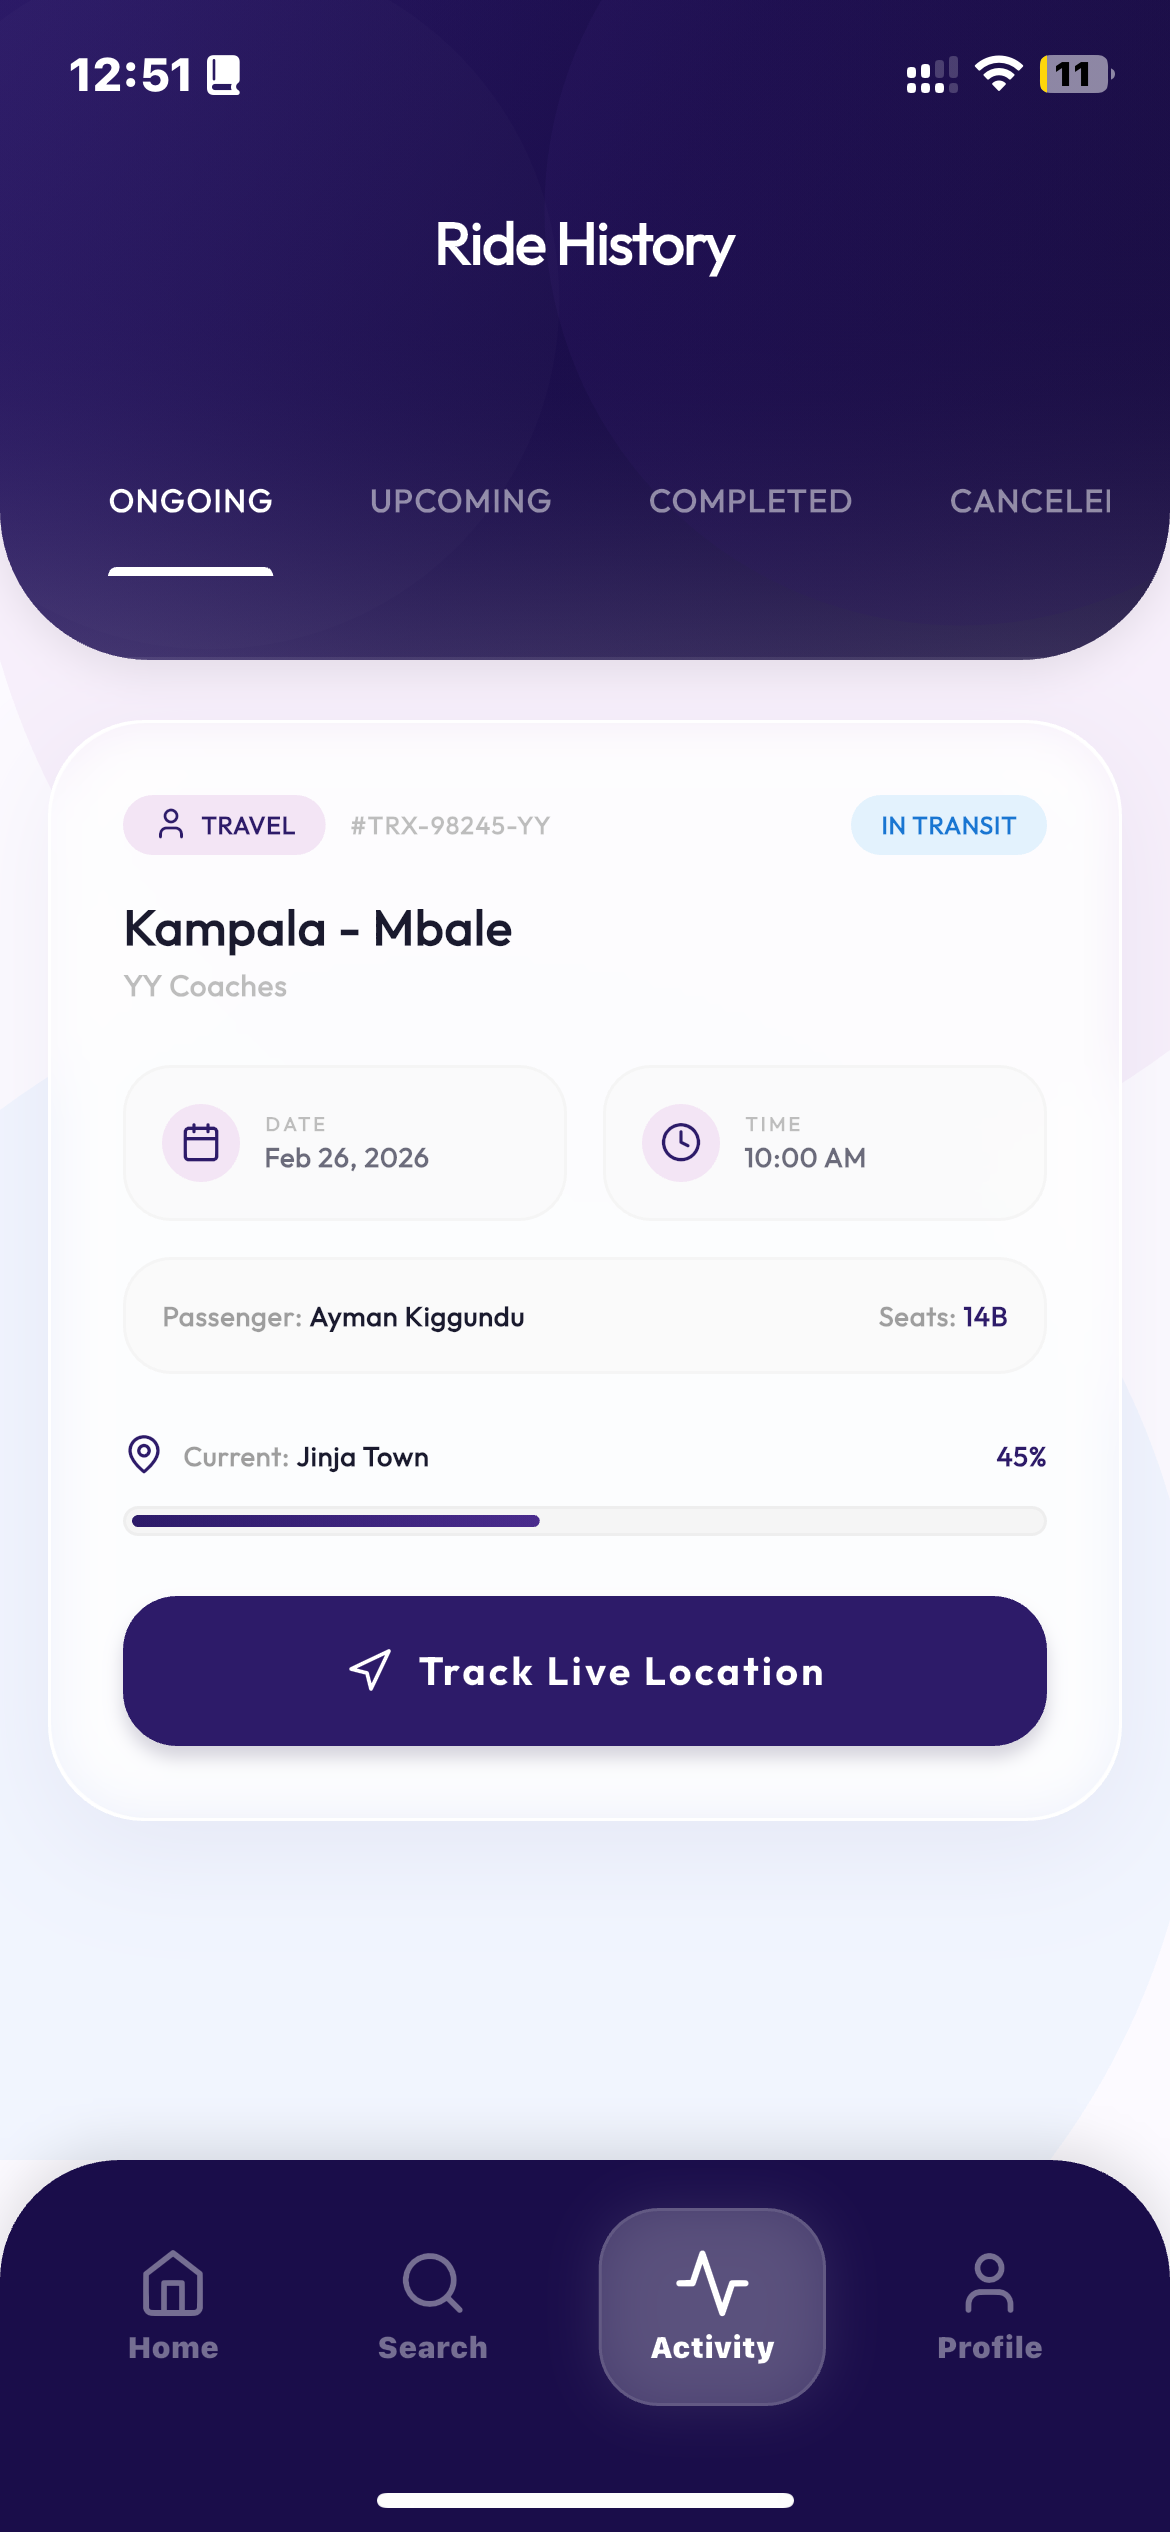
\includegraphics[width=\linewidth]{images/FYP/Ongoing trip tracking.PNG}
    \caption{Ongoing trip tracking}
\end{subfigure}
\hfill
\begin{subfigure}{0.32\textwidth}
    \centering
    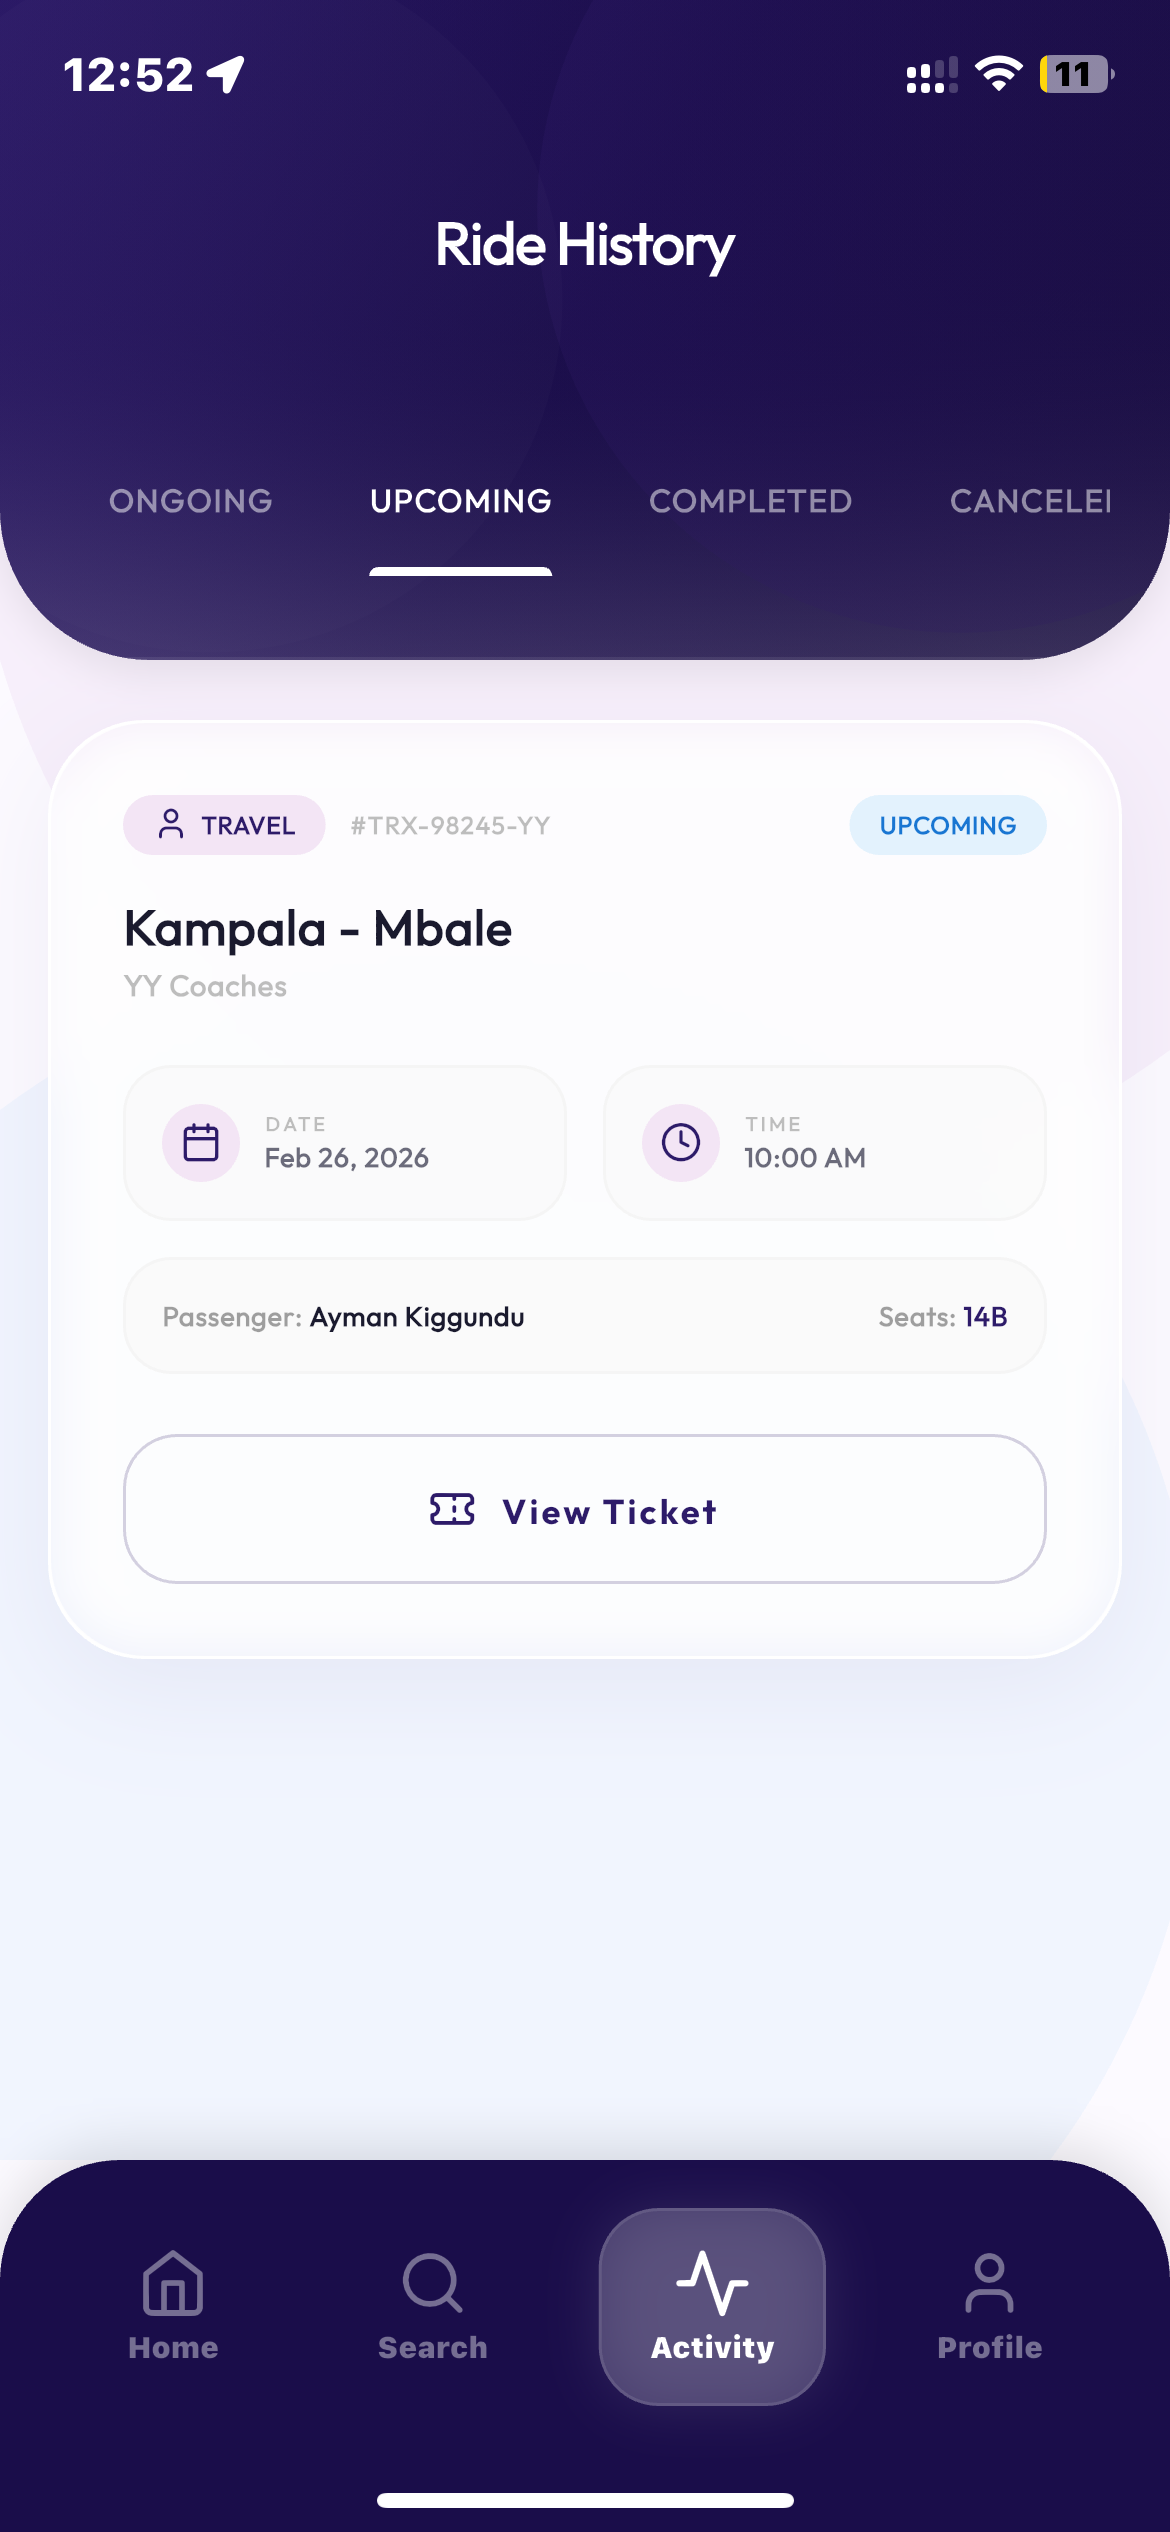
\includegraphics[width=\linewidth]{images/FYP/Tracking upcoming trips.PNG}
    \caption{Tracking upcoming trips}
\end{subfigure}
\hfill
\begin{subfigure}{0.32\textwidth}
    \centering
    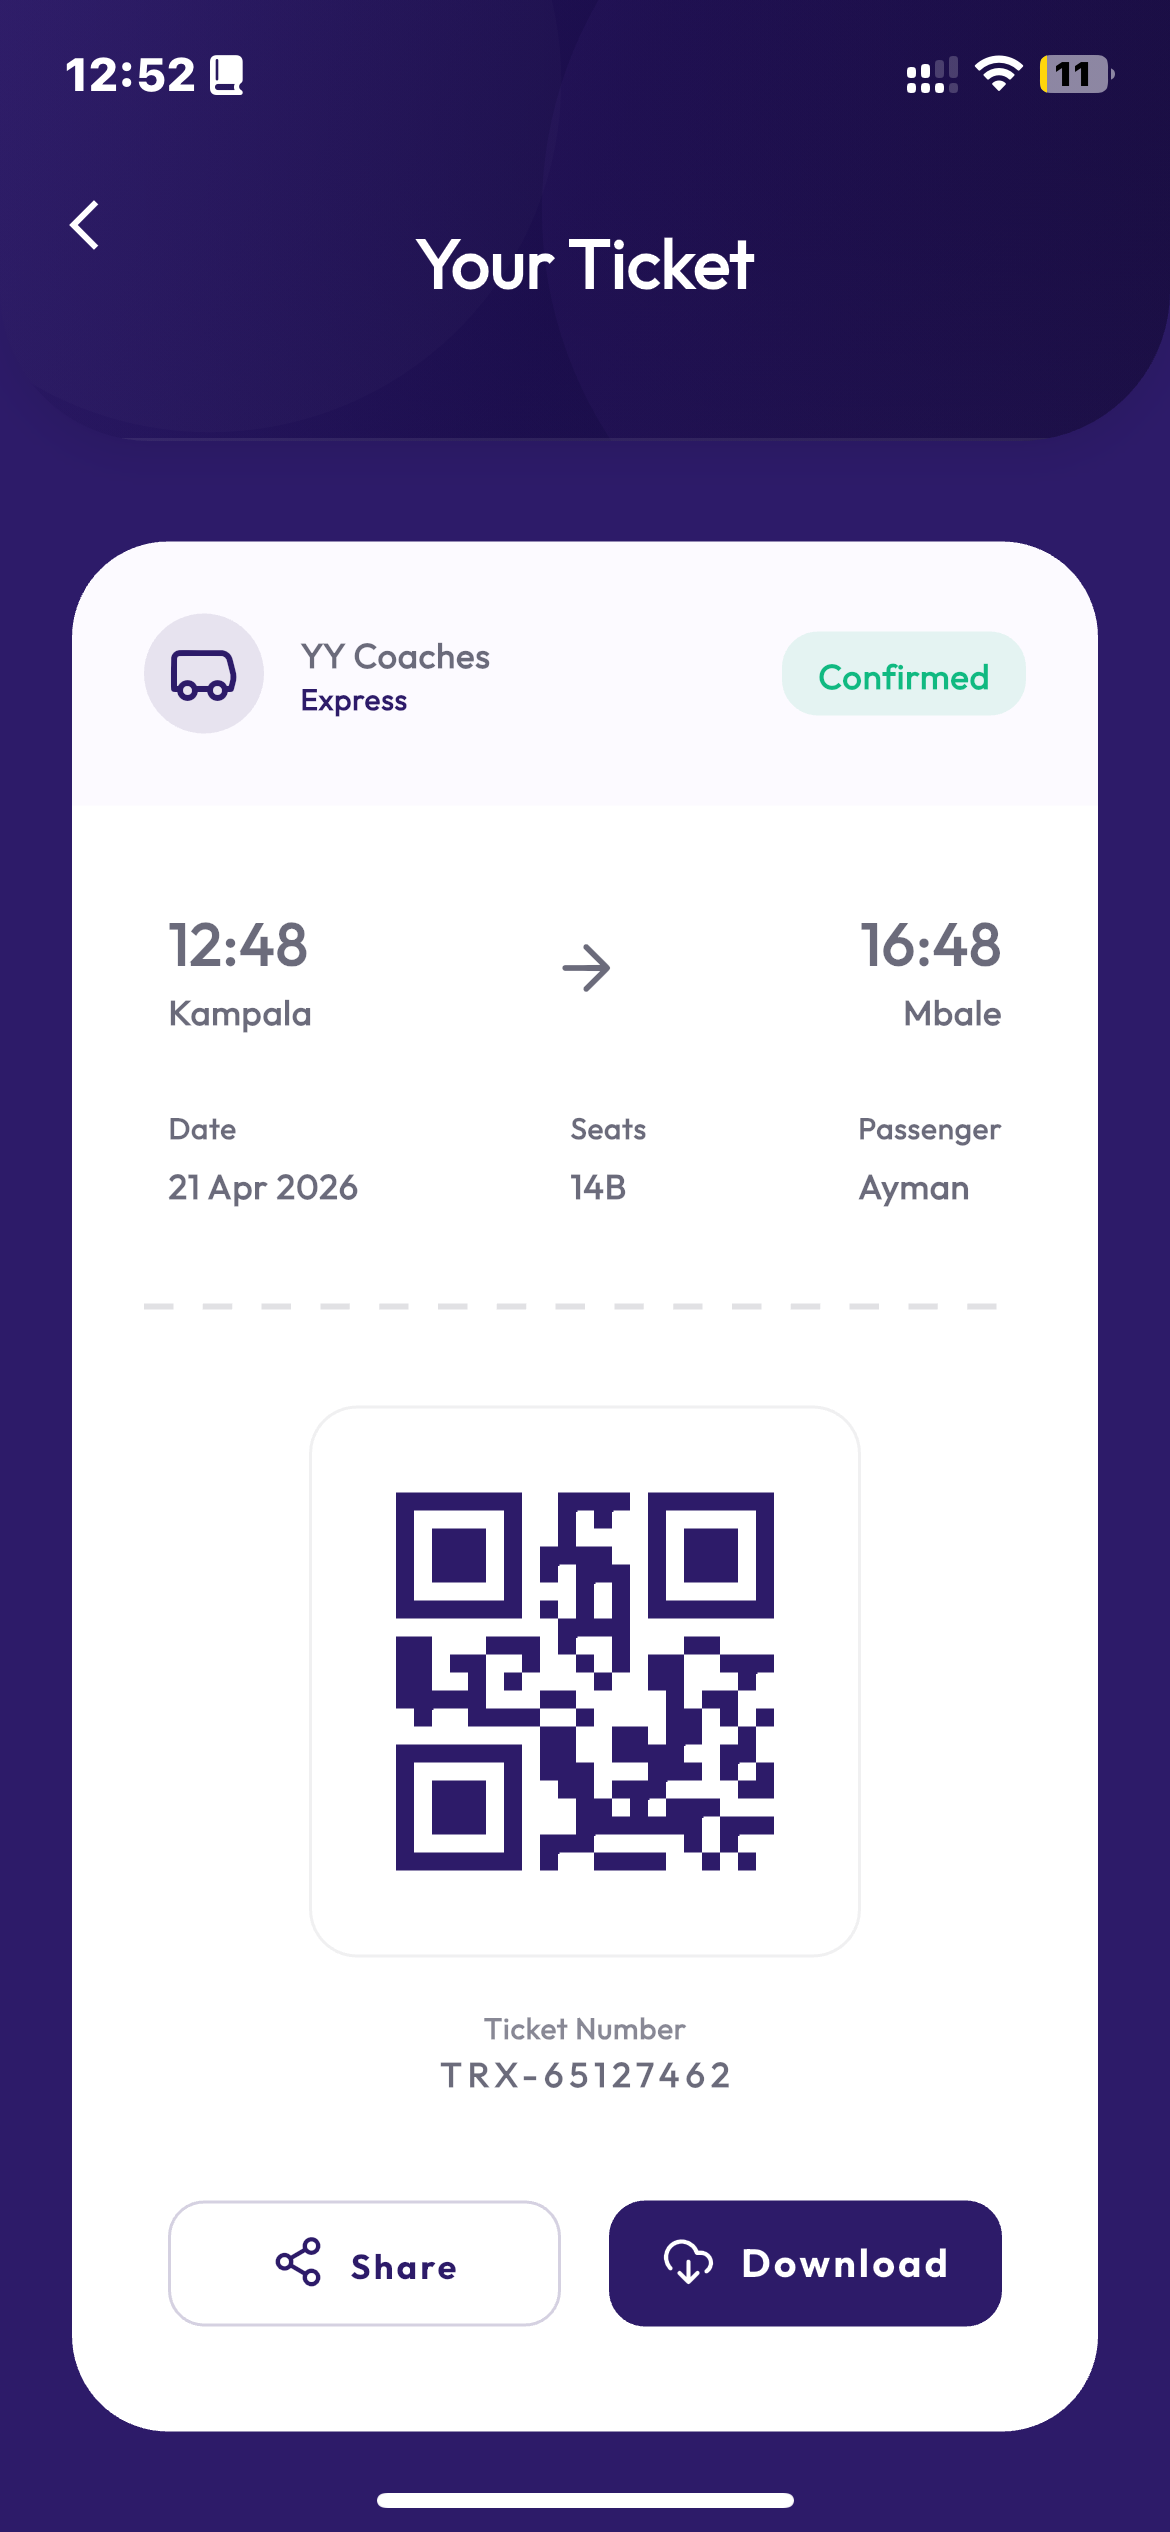
\includegraphics[width=\linewidth]{images/FYP/Digital Ticket.PNG}
    \caption{Digital ticket}
\end{subfigure}

\caption{Operator interfaces}
\label{fig:passenger-interfaces}

\end{figure}

\subsection{System Testing and Validation}
To ensure a robust and reliable system, testing was performed continuously at every stage of development. The approach emphasizes early detection of defects and validation of functionality rather than deferring testing until the end of the project. This proactive
strategy guarantees that issues are identified and resolved promptly, maintaining high system
quality and reliability. 

\subsection{Testing strategy and tools}
The system underwent multiple layers of testing, covering individual components, integration points, overall system performance, and real-world usability:

\textbf{Unit testing}: Individual components were validated using unit tests to ensure that
each module behaved as expected in isolation. For the backend, pytest was used to test Python and Django functionality, while the frontend Flutter applications employed flutter test and mockito for widget and logic testing. The development goal was to achieve greater than eighty five percent coverage on critical paths, ensuring that essential features functioned reliably under a variety of conditions.

\textbf{Integration testing}: Integration tests verified that different modules interacted correctly and that API contracts were honored. Backend APIs were tested using structured Postman collections to ensure correct request-response behavior, while end-to-end flows for
mobile applications were tested using the Flutter Integration Driver. This ensured that
data flowed seamlessly between clients, the backend, and external services.

\textbf{System and Load Testing}: To evaluate system performance under realistic usage conditions, load tests simulated up to 200 concurrent driver and passenger sessions using tools such as k6 or Locust. Performance metrics, including GPS update latency, were monitored to confirm that updates remained under 4 seconds even on 3G networks. These tests validated the system’s scalability, responsiveness, and resilience under peak loads.

\textbf{Real-World Field Testing}: 
Controlled simulations alone were not sufficient to capture the practical challenges faced in private shuttle operations, particularly those identified during the interview with HillsLink Express. Instead, the system design and evaluation were guided by real-world operational scenarios derived from the interview findings.

These scenarios included common activities such as seat booking via phone, managing no-shows, handling mid-route passenger drop-offs, coordinating parcel deliveries, and responding to frequent customer inquiries about vehicle location and delivery status. By modelling these real-life interactions within the Traxis system, the study was able to assess how effectively the proposed solution addresses existing inefficiencies.

This approach ensured that the system was grounded in actual user needs and operational constraints, including limited digital literacy, reliance on phone communication, and the need for flexible booking and tracking mechanisms. As a result, Traxis was evaluated based on its ability to improve coordination, enhance transparency, and reduce operational burden within the context of private shuttle services.

\textbf{User Acceptance Testing (UAT)}: Finally, the system underwent UAT(User Acceptance Tests) with a Hillslink passenger alongside the operator. Participants performed typical tasks using the system over a two-week period. Think-aloud sessions and standardized questionnaires such as the SUS(System Usability Scale) were employed to capture qualitative and quantitative feedback, validating that the system met user needs and expectations.
The testing strategy leveraged a variety of professional tools, including Postman for API testing, Flutter DevTools for debugging and performance profiling,
Firebase Test Lab for real-device testing, Sentry for crash reporting from the earliest stages of development, and Firebase Performance Monitoring for continuous perfor
mance evaluation. 

By employing this comprehensive, multi-layered testing and validation strategy, the
Traxis system achieved high reliability, responsiveness, and usability, ensuring readiness for real-world deployment and sustained user satisfaction

